\documentclass{beamer}
\usepackage[utf8]{inputenc}

% Theme and Color Scheme
\usetheme{Madrid}
\usecolortheme{default}

% Essential Packages
\usepackage{amsmath,amssymb,amsfonts,amsthm}
\usepackage{txfonts}
\usepackage{graphicx}
\usepackage{listings}
\usepackage{gvv} % For \myvec command
\usepackage{lmodern}
\usepackage{tikz}
\usepackage{tkz-euclide}

% For code listings
\usepackage{tcolorbox}
\tcbuselibrary{minted,breakable,xparse,skins}

% Page Numbering
\setbeamertemplate{page number in head/foot}[totalframenumber]

% Custom color for code background
\definecolor{bg}{gray}{0.95}

% C language style for listings
\lstset{
    language=C,
    basicstyle=\ttfamily\small,
    keywordstyle=\color{blue},
    stringstyle=\color{orange},
    commentstyle=\color{green!60!black},
    numbers=left,
    numberstyle=\tiny\color{gray},
    breaklines=true,
    showstringspaces=false,
}
%------------------------------------------------------------
%This block of code defines the information to appear in the
%Title page
\title %optional
{1.9.5}
\date{September 16, 2025}
%\subtitle{A short story}

\author % (optional)
{Taraka Abhinav - EE25BTECH11016}


\begin{document}

% FRAME 1: Title Page
\frame{\titlepage}

% FRAME 2: Question
\begin{frame}{Question}
Find the distance between the points $(0,2\sqrt{5})$ and $(-2\sqrt{5},\,0)$.
\end{frame}

% FRAME 3: Theoretical Solution - Setup
\begin{frame}{Theoretical Solution}
Let the points be $\vec{A} = (0,2\sqrt{5})$ and $\vec{B} = (-2\sqrt{5},0)$.
\begin{align}
\vec{A} &= \myvec{0\\2\sqrt{5}}, \quad 
\vec{B} = \myvec{-2\sqrt{5}\\0}
\end{align}
The distance between two points is given by
\begin{align}
d &= \norm{\vec{A}-\vec{B}}
\end{align}
\end{frame}

% FRAME 4: Theoretical Solution - Substitution
\begin{frame}{Theoretical Solution}
Substituting values,
\begin{align}
d &= \norm{\myvec{0\\2\sqrt{5}}-\myvec{-2\sqrt{5}\\0}} \\ 
  &= \norm{\myvec{2\sqrt{5}\\2\sqrt{5}}} \\ 
  &= \sqrt{(2\sqrt{5})^2 + (2\sqrt{5})^2}
\end{align}
Simplifying,
\begin{align}
d &= \sqrt{20 + 20} \\
  &= \sqrt{40} \\
  &= 2\sqrt{10}
\end{align}
\begin{align}
\implies d = \boxed{2\sqrt{10}}
\end{align}
\end{frame}


% FRAME 5: C Code
\begin{frame}[fragile]
    \frametitle{C Code - Distance Formula}
    \begin{lstlisting}
#include <stdio.h>
#include <stdlib.h>
#include <math.h>

// Function to compute distance between (x1,y1) and (x2,y2)
double find_distance(double x1, double y1, double x2, double y2) {
    double dx = x2 - x1;
    double dy = y2 - y1;
    return sqrt(dx*dx + dy*dy);
}

int main() {
    double x1 = 0, y1 = 2*sqrt(5);
    double x2 = -2*sqrt(5), y2 = 0;
    double d = find_distance(x1, y1, x2, y2);
    printf("Distance = %.4f\n", d);
    return 0;
}
    \end{lstlisting}
\end{frame}

% FRAME 6: Python + C Code
\begin{frame}[fragile]
    \frametitle{Python + C Code}
    \begin{lstlisting}[language=Python]
import ctypes
import numpy as np
import matplotlib.pyplot as plt
import math

# Load shared library
lib = ctypes.CDLL('./section.so')

# Define function signature
lib.find_distance.argtypes = [ctypes.c_double, ctypes.c_double,
                             ctypes.c_double, ctypes.c_double]
lib.find_distance.restype = ctypes.c_double

# Points
x1, y1 = 0, 2*math.sqrt(5)
x2, y2 = -2*math.sqrt(5), 0

# Call C function
dist = lib.find_distance(x1, y1, x2, y2)
print(f"Distance = {dist:.2f}")
    \end{lstlisting}
\end{frame}

% FRAME 7: Python + C Code (Plotting)
\begin{frame}[fragile]
    \frametitle{Python + C Code}
    \begin{lstlisting}[language=Python]
# Define points
A = np.array([x1, y1])
B = np.array([x2, y2])

# Plot line AB and points
plt.plot([A[0], B[0]], [A[1], B[1]], 'k-', label='$AB$')
plt.scatter([A[0], B[0]], [A[1], B[1]], c=['red', 'blue'])

# Annotate points
labels = [f"A({x1},{y1:.2f})", f"B({x2:.2f},{y2})"]
for label, coord in zip(labels, [A, B]):
    plt.annotate(label, (coord[0], coord[1]),
                 textcoords="offset points",
                 xytext=(10, -10), ha='center')

# Decorations
plt.legend()
plt.grid(True)
plt.axis('equal')
plt.title(f"Distance = {dist:.2f}")
plt.savefig("2.png", dpi=150)
plt.show()
    \end{lstlisting}
\end{frame}

% FRAME 8: Python Code
\begin{frame}[fragile]
    \frametitle{Python Code}
    \begin{lstlisting}[language=Python]
import numpy as np
import matplotlib.pyplot as plt

# Define the points
A = np.array([0, 2*np.sqrt(5)])
B = np.array([-2*np.sqrt(5), 0])

# Compute distance
dx = B[0] - A[0]
dy = B[1] - A[1]
distance = np.sqrt(dx**2 + dy**2)
print(f"Distance = {distance:.2f}")

# Plot line AB
plt.plot([A[0], B[0]], [A[1], B[1]], 'k-',
         label=f'Distance = {distance:.2f}')
    \end{lstlisting}
\end{frame}

% FRAME 9: Python Code (Plotting)
\begin{frame}[fragile]
    \frametitle{Python Code}
    \begin{lstlisting}[language=Python]
# Plot points
plt.scatter([A[0], B[0]], [A[1], B[1]], c=['red', 'blue'])
labels = [f'A(0, 2√5)', f'B(-2√5, 0)']
coords = [A, B]

# Annotate points
for label, coord in zip(labels, coords):
    plt.annotate(label,
                 (coord[0], coord[1]),
                 textcoords="offset points",
                 xytext=(10, -10),
                 ha='center')
# Decorations
plt.legend()
plt.grid(True)
plt.axis('equal')
plt.title("Distance between Two Points")
plt.savefig("distance_plot.png", dpi=150)
plt.show()
    \end{lstlisting}
\end{frame}

% FRAME 10: Plot
\begin{frame}{Plot}
    \centering
    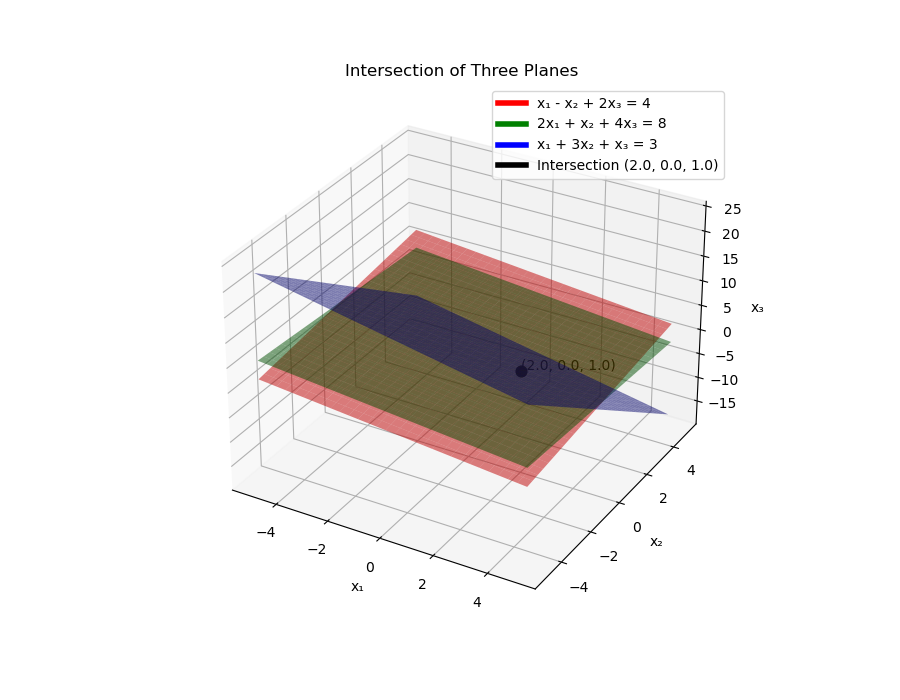
\includegraphics[width=0.8\columnwidth]{beamer/figs/Figure_1.png}     
\end{frame}

\end{document}